%% Uji Fase 3: seluruh halaman bagian awal + lampiran.
%% Kompilasi: pdflatex -interaction=nonstopmode uji-fase3.tex  (2x, daftar isi perlu 2 pass)
\documentclass[jenis=skripsi,mode=laporan,jenjang=sarjana,sitasi=apa,
               logodir=../logo,logo=logo-placeholder]{unnes-ta}

\identitas{
  judul      = {Pengembangan Media Pembelajaran Berbasis Augmented Reality untuk
                Meningkatkan Hasil Belajar Siswa Sekolah Menengah Kejuruan},
  nama       = {Nama Mahasiswa},
  nim        = {1234567890},
  prodi      = {Pendidikan Teknik Informatika},
  fakultas   = {Fakultas Teknik},
  gelar      = {Sarjana Pendidikan},
  tahun      = {2026},
  pembimbinga    = {Dr. Pembimbing Satu, M.Kom.},
  pembimbinganip = {198001012005011001},
  pembimbingb    = {Dr. Pembimbing Dua, M.Pd.},
  pembimbingbnip = {198502022010012002},
  ketua        = {Prof. Dr. Ketua Penguji, M.Pd.},
  ketuanip     = {196001011990031001},
  sekretaris   = {Dr. Sekretaris Penguji, M.Kom.},
  sekretarisnip= {197002022000031002},
  penguji1     = {Dr. Penguji Satu, M.Pd.},
  penguji1nip  = {197503032005012003},
  penguji2     = {Dr. Penguji Dua, M.Kom.},
  penguji2nip  = {198004042010011004},
  penguji3     = {Dr. Pembimbing Satu, M.Kom.},
  penguji3nip  = {198001012005011001},
  hari         = {Senin},
  tanggal      = {12 Januari},
  tanggalpersetujuan = {10 Januari 2026},
  tanggalpernyataan  = {10 Januari 2026},
  tempatlahir  = {Semarang},
  tanggallahir = {1 Januari 2004},
  alamat       = {Jalan Contoh Nomor 1, Sekaran, Gunungpati, Semarang},
  surel        = {nama.mahasiswa@students.unnes.ac.id},
}

\begin{document}
\bagianawal

\sampul
\halamanjudul
\punggung

\persetujuanpembimbing
\pengeshantimpenguji
\pernyataankeaslian

\motopersembahan{%
  \begin{center}
    ``Ilmu tanpa amal bagaikan pohon tanpa buah.''\\[0.4cm]
    \textit{(pepatah)}
  \end{center}
  \vspace{0.6cm}
  \noindent Persembahan: karya ini dipersembahkan untuk kedua orang tua, keluarga, dan
  almamater Universitas Negeri Semarang.
}

\abstrak[media pembelajaran, augmented reality, hasil belajar]{%
  Tujuan penulisan tugas akhir ini adalah mengembangkan media pembelajaran berbasis
  \textit{augmented reality} dan menguji keefektifannya terhadap hasil belajar siswa.
  Metode yang digunakan adalah penelitian pengembangan dengan model ADDIE yang meliputi
  analisis, perancangan, pengembangan, implementasi, dan evaluasi. Subjek uji coba adalah
  36 siswa kelas XI. Hasil pengembangan berupa aplikasi yang valid menurut ahli media dan
  ahli materi, serta efektif meningkatkan hasil belajar dengan n-gain sedang.
}

\abstracten[learning media, augmented reality, learning outcomes]{%
  This final project aimed to develop augmented reality based learning media and to examine
  its effect on student learning outcomes. The study employed the ADDIE development model
  covering analysis, design, development, implementation, and evaluation. The subjects were
  36 eleventh grade students. The product was valid according to media and subject matter
  experts and effective in improving learning outcomes with a moderate n-gain.
}

\begin{prakata}
Puji syukur penulis panjatkan atas selesainya penyusunan tugas akhir ini. Ucapan terima
kasih disampaikan kepada dosen pembimbing, keluarga, serta rekan mahasiswa yang telah
membantu kelancaran penyusunan karya ini.
\end{prakata}
\tandatanganprakata{Penulis}

\daftarisi
\daftargambar
\daftartabel

\daftaristilah{%
  \istilah{AR}{Augmented Reality, teknologi yang menyisipkan objek maya ke dunia nyata}
  \istilah{ADDIE}{Analysis, Design, Development, Implementation, Evaluation}
  \istilah{N-gain}{nilai peningkatan hasil belajar sebelum dan sesudah perlakuan}
}

\daftarlampiran

\bagianutama
\chapter{PENDAHULUAN}
\section{Latar Belakang}
Bab ini menguraikan alasan penelitian melalui pemaparan fenomena yang ditemui peneliti
beserta kesenjangan antara kondisi nyata dan kondisi yang seharusnya, sekaligus menunjukkan
kebaruan penelitian dibandingkan penelitian terdahulu yang relevan.

\begin{table}[htbp]
  \centering
  \caption{Ringkasan penelitian terdahulu yang relevan}
  \label{tab:terdahulu}
  \begin{tabular}{clc}
    \toprule
    No & Fokus penelitian & Hasil \\
    \midrule
    1 & Media berbasis AR & Efektif pada ranah kognitif \\
    2 & Hasil belajar SMK & Meningkat kategori sedang \\
    \bottomrule
  \end{tabular}
  \sumber{Penelitian terdahulu yang diolah penulis (2026)}
\end{table}

\begin{figure}[htbp]
  \centering
  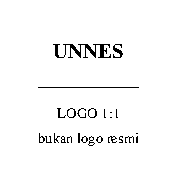
\includegraphics[width=3cm]{../logo/logo-placeholder}
  \caption{Kerangka berpikir penelitian}
  \label{gam:kerangka}
  \sumber{Dokumentasi penulis}
\end{figure}

\chapter{PENUTUP}
\section{Simpulan}
Simpulan memuat jawaban atas tujuan penelitian yang telah dirumuskan pada bab pendahuluan.

\lampiranbuktiizinpenelitian
\lampiraninstrumen
\lampiranizinetik
\lampiranskpembimbing
\lampiranskpenguji
\biodatapenulis{%
  \textbf{Riwayat Pendidikan}\par
  \begin{enumerate}
    \item SD Negeri Contoh, lulus tahun 2016.
    \item SMP Negeri Contoh, lulus tahun 2019.
    \item SMA Negeri Contoh, lulus tahun 2022.
    \item Universitas Negeri Semarang, Program Studi Pendidikan Teknik Informatika.
  \end{enumerate}
}
\end{document}
